\section{Background and Motivation}
\label{sec:background}
The organization question begins with the dependency graph. We first identify
its recurring structure and numerical variants, then use measured and analytical
examples to derive the requirements for a common method.

\subsection{Butterfly computation and its variants}
A butterfly computation combines small groups of values through a sequence
of stages. In a radix-two stage, disjoint pairs can execute independently,
but the next stage pairs their outputs differently. These changing partners
are what make local computation easy to parallelize and the complete
computation difficult to organize.
For $N=2^L$, the graph has $L$ stages and $N/2$ pair
updates per stage. A stage associated with bit $q$ pairs indices $i$ and
$i\mathbin{\oplus}2^q$. The stage sequence defines the dependency envelope,
while the pair function supplies arithmetic and coefficients. Batch instances
add independent copies of the graph. \textbf{Shared structure does not imply
interchangeable semantics.}

The family includes complex FFT, finite-field NTT, sum-and-difference FWHT,
subset and superset zeta transforms, and products of structured $2\times2$
stages. One-sided zeta updates use a subset of the full pairing dependencies.
For example, an FFT pair multiplies by a complex twiddle, an NTT pair performs
modular arithmetic, and an FWHT pair uses only sums and differences. A common
organization must retain these distinctions rather than replace every pair
with one arithmetic implementation. Multidimensional separable transforms
compose axis transforms with a shared tensor layout, making inter-axis
placement part of the same execution problem.

Cooley--Tukey (CT) and Gentleman--Sande (GS) illustrate another distinction
~\cite{cooley1965,gentleman1966}. Their local forms place twiddle
multiplication on opposite sides of addition and subtraction. Forward and
inverse computation also change coefficients, stage order, permutations, and
normalization. Stockham algorithms distribute permutations across passes
~\cite{stockham1966}. Section~\ref{sec:equivalence} explains which structural
relations survive these changes.

The requested precision, direction, normalization, and input/output layout
constrain implementation choices. Internal reordering is legal only when it
preserves the request, with adaptation included in execution cost.

\textbf{The same graph admits different organizations.}
Figure~\ref{fig:organization-tradeoffs} holds the 16-point Hadamard graph
fixed. Stagewise execution exposes eight independent pairs and transfers all
values at every stage. Two-stage bands retain four values per region and halve
materialized traffic. A whole-transform band minimizes traffic but exposes
one independent region per transform. These region counts do not fix worker
counts, since workers can cooperate within a region.

\begin{figure}[t]
\centering
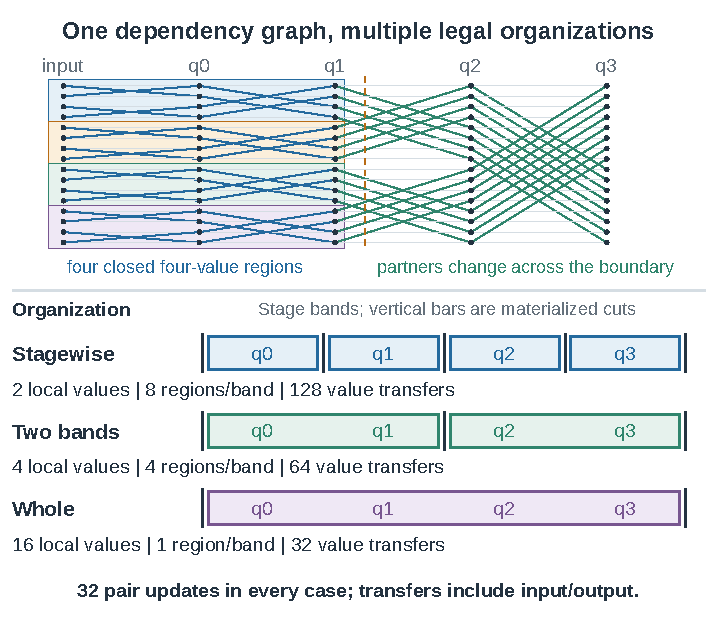
\includegraphics[width=\columnwidth]{figures/drawio/exports/organization_tradeoffs.pdf}
\caption{Grouping stages trades local state and independent regions for
fewer transfers in the same Hadamard graph. Counts are analytical.}
\label{fig:organization-tradeoffs}
\end{figure}

Storage scopes give these logical choices physical costs~\cite{ampere}.
Worker-local storage, shared storage, and external storage offer different
capacities and exchange rates. A generated codelet or imported core such as
cuFFTDx~\cite{cufftdx} must operate within those limits. The preferred grouping
therefore depends on both arithmetic service and the surrounding organization.
